\section{Demonstration}
% Organize this section according to major topics
% give each topic a section heading in boldface.
% try to cover the major common points :
%
% problem design
% methods of measurement
% supporting models
% supporting data
% simulations run
% results

% Just write the section headings for each part and indicate what goes in that
% section with words :
%
% heading
% figures (with captions)
% schematics (with captions and footnotes)
% equations
% tables

% What does it mean?
% What did I actually test?
% What were the results?
% Did the work yield a new method?
% Did the work yield new knowledge?
% What measurements did I make?
% How were these measurements characterized?
% What methods were used?
% What were the results?
% How were the measurements made and characterized?


The success of the \Cyclus simulator can be measured in many ways.  The most
compelling are demonstrations of fundamental simulation capability and of the
feasibility of the \Cyclus community-driven development model. Nascent promising
growth of the \Cyclus ecosystem at multiple institutions indicates that a fuel
cycle simulator can advance in this community-driven development
paradigm. Additionally, simulation results for both once-through and more
complex recycling scenarios demonstrate that \Cyclus possesses the fundamental
fuel cycle simulation capabilities to contribute to the field.

\subsection{Ecosystem}
% Cycamore library
% Cyder?

The \Cyclus community-driven software development model seeks to break the
unproductive proliferation of overspecialized simulators. It instead leverages
the collective expertise of fuel cycle researchers toward a single, more
extensible, tool. Through the targeted
contributions of those researchers, an ecosystem of capabilities should emerge.
The \Cyclus `Ecosystem' is the collection of tools, calculation libraries,
archetypes, data, and input files intended for use with the \Cyclus simulator.
Members of the ecosystem include:
\begin{itemize}
\item the archetypes provided in the \Cycamore \cite{carlsen_cycamore_2014}
repository
\item the archetypes created by researchers
\item isotopic composition data
\item historical facility deployment data
\item the \Cyclus \gls{GUI} tool Cyclist
\item fundamental analysis tools in the \Cyclus toolkit
\item tools for \Cyclus optimization, parallelization, and development
\end{itemize}
Taken together, these form an ecosystem of capabilities. Over time, this
ecosystem will grow as archetype developers, kernel developers, and
even users contribute capabilities developed for their own needs. Indeed, the
long-term vision for the \Cyclus framework predicts an ever-expanding ecosystem
of both general and specialized capability extensions.

Already, the ecosystem is growing. Early cross-institutional contributions to
the ecosystem demonstrate a significant achievement by the \Cyclus framework
and provide the basis for a community-driven development model.

\subsubsection{Supplementary Projects}

A number of projects and tools outside of the core simulation kernel have been
developed to improve the scope and the diversity of the capabilities in the
\Cyclus ecosystem. Table \ref{tab:coretools} lists the tools and projects
developed under close integration with the \Cyclus kernel.  These tools are used
to ease development and simulation design (Cycstub, Cycic, Ciclus), data
visualization and analysis (Cyclist, Cyan), and remote execution (Cloudlus).

\begin{table}[h]
\centering
\begin{tabularx}{\textwidth}{|r|X|r|}
\hline
\textbf{Name} & \textbf{Description} & \textbf{Citation} \\
\hline
Cycic &  Input control - embedded in Cyclist & \cite{flanagan_input_2013}\\
Cyclist & Interactive data exploration environment & \cite{livnat_cyclist_2014} \\
Ciclus & Continuous integration scripts for \Cyclus & \cite{scopatz_ciclus_2014}\\
Cycstub & Skeleton for clean slate module development & \cite{carlsen_cycstub_2014}\\
Cyan & \Cyclus analysis tool & \cite{carlsen_cyan_2014}\\
Cloudlus & Tools for running \Cyclus in a cloud environment & \cite{carlsen_cloudlus_2014} \\
\hline
\end{tabularx}
\caption{Many tools have been developed outside of the scope of the \Cyclus kernel for improved user, developer, and analyst experiences with \Cyclus.}
\label{tab:coretools}
\end{table}

\subsubsection{Archetype Contributions}

It is expected that the most common type of contribution to \Cyclus will be
contributions of new archetypes. Researchers will be driven to create a new
archetype when a need arises, such as to improve the fidelity of simulation,
or to represent a novel reactor type, an innovative
reprocessing strategy, or a particular governmental or institutional behavior.
The real-world utility of \Cyclus can in part be measured by the breadth and
diversity of archetypes being developed in this way.

Early progress has been promising. Many archetypes external to the \Cycamore
library (Table \ref{tab:cycamore}) have been
\cite{huff_streamblender_2014,huff_commodconverter_2014} or are being
\cite{flanagan_bright-lite_2014,skutnik_nuclear_2014,huff_mktdriveninst_2014}
developed for contribution to the \Cyclus ecosystem. These archetypes provide
the first examples of developer-contributed capabilities.  They add to the
fundamental \Cycamore archetypes by providing physics-based reactors,
separations logic, fuel fabrication processing, storage facilities, and expanded
institutional paradigms.  The existence and diversity of these contributed
archetypes illustrate the power and potential of the community-based development
approach that \Cyclus has taken.


\begin{table}[h]
\centering
\begin{tabularx}{\textwidth}{|r|X|r|}
\hline
\textbf{Name} & \textbf{Description} & \textbf{Citation} \\
\hline
Bright-lite & A physics-based reactor archetype and fuel fabrication archetype & \cite{flanagan_bright-lite_2014} \\
Nuclear Fuel Inventory Model & A flexible, ORIGEN-based, reactor analysis module & \cite{skutnik_nuclear_2014} \\
CommodConverter & A simple commodity converting storage facility archetype  & \cite{huff_commodconverter_2014} \\
MktDrivenInst & An institution that controls deployment based on commodity availability & \cite{huff_mktdriveninst_2014} \\
SeparationsMatrix & A facility for elemental separations of used fuel & \cite{huff_streamblender_2014} \\
StreamBlender & A facility for fuel fabrication from reprocessed streams & \cite{huff_streamblender_2014} \\
\hline
\end{tabularx}
\caption{A diverse set of archetypes under development reflect the diverse
needs of researchers at various institutions. These archetypes, contributed
outside of the \Cyclus core and \Cycamore libraries are the first demonstration
of community-driven development in a fuel cycle simulator.}
\label{tab:archetypes}
\end{table}

\subsection{Simulations}
\label{ref:simulation}
%Inpro example (is this still running or did we deprecate it with 1.0?)

% MJG - INPRO should be tried again. @rwcarlsen has been running lots of
% simulations with the batch reactor, and its the second generation of my
% reactor models. We could easily use the same demand schedule and enrichment
% facility parameters and run it again.

This section will discuss the creation and results of a few simple fuel cycle
simulations to help illustrate the flexibility of \Cyclus. These simulations are
designed to illustrate Cyclus' capability.  Many simplifying assumptions have
been made with respect to material compositions, fuel transmutation, among
others. The three fuel cycles examined are:

\begin{enumerate}
    \item Once through (no recycle)
    \item 1-pass \gls{MOX} recycle
    \item Infinite-pass \gls{MOX} recycle
\end{enumerate}

For each of these fuel cycles, a 1,100 month single-reactor \Cyclus simulation
was run in addition to a 10-reactor simulation with staggered refueling times.
As the number of staggered-cycle reactors increases the system converges
toward continuous material flow results.  \Cyclus flexibility allows this
transition to be examined.  The facilities used in these simulations are:

\begin{itemize}

    \item \textbf{Reactor} (\Class{cycamore::Reactor}): This is a reactor
        model that requests any number of input fuel types and transmutes them
        to static compositions when they are burnt and discharged from the
        core. The reactor was configured to model a light water reactor
        with a 3 batch core (20,000 kg HM per batch) operating on an 18 month
        cycle with a 2 month refuel time.  The reactor was also configured to
        take in either enriched \gls{UOX} fuel or recycled \gls{MOX} fuel.

    \item \textbf{Recycled Fuel Fabrication} (\Class{cycamore::Fab}): This
        facility requests depleted uranium and separated fissile material and
        mixes them together into recycled \gls{MOX} fuel that it offers to
        requesters.  The two streams are mixed in a ratio in order to match
        simple neutronics properties of the target fuel as closely as
        possible.  The method used is based on a variation "equivalence
        method" originally developed by Baker and Ross
        \cite{baker_comparison_1963}.  This technique has also been used in the
        \gls{COSI} fuel cycle simulator developed by the French \gls{CEA}.

    \item \textbf{Separations} (\Class{cycamore::Separations}): This facility
        takes in all kinds of spent fuel and separates it into plutonium and
        waste streams with some efficiency (0.99 was used for these
        simulations).  Up to 60,000 kg of Pu can be separated per month.

    \item \textbf{Repository} (\Class{cycamore::Sink}): This is an
        infinite-capacity facility that can take in all types of material
        including separations waste streams and spent reactor fuel.

    \item \textbf{UOX Fabrication} (\Class{cycamore::Source}): This facility
        provides enriched \gls{UOX} fuel as requested.  This facility has infinite
        production capacity.

    \item \textbf{DU Source} (\Class{cycamore::Source}): This facility
        provides depleted uranium as requested. This facility has infinite
        production capacity.

\end{itemize}

Modifying the input file specification to model each of the 3 fuel cycles was
done by making simple adjustments to the commodities and trade preferences for
each of the facilities.  The reactor was configured to request recycled \gls{MOX}
fuel with a higher preference than new \gls{UOX} fuel. For the once through case,
the \Class{Reactor} was set to offer all spent fuel as waste.  For the 1-pass
recycle case, the \Class{Reactor} offered spent \gls{UOX} into a spent fuel market,
but spent \gls{MOX} is still offered as waste.  In the infinite-pass recycle case,
the \Class{Reactor} offers all burned fuel into a spent fuel market. The
separations facility requests spent fuel with a higher preference than the
repository resulting in preferential recycle.  All these preferences are easy
to adjust and \Cyclus dynamically handles supply constraints and non-uniform
preference resolution.  It is notable that separations and recycle fuel
fabrication capacity are deployed identically in all simulations.  In the once
through case, the recycling loop never acquires material, and so reactors
always receive fresh \gls{UOX} fuel.  The \gls{DRE} ensures everything operates
smoothly in all cases.

Cyclus' discrete materials make single-pass recycle straightforward to implement.  The
reactors keep track of fuel as discrete batches. A reactor remembers where it
received each batch from.  If a batch was received from the recycled fuel
fabrication facility, it does not offer it to separations and instead offers
it as a waste commodity which is only requested by the repository.  The
material flows for the 1-pass recycle case are shown in Figure
\ref{fig:flowmodopen}.

\begin{figure}[H]
\begin{center}
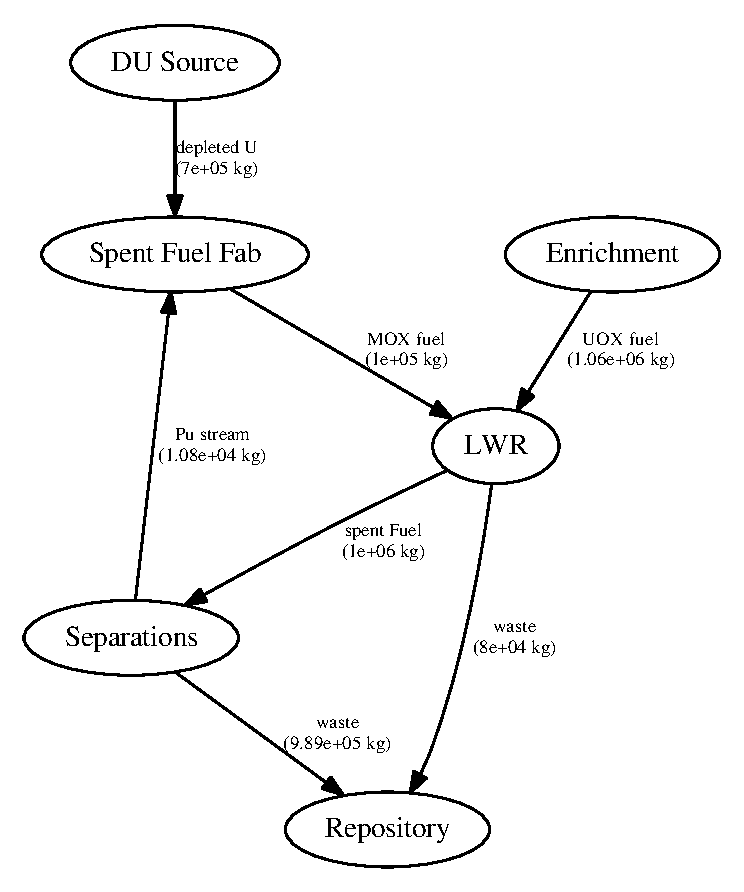
\includegraphics{./images/flow-mod-open-1.eps}
\end{center}
\caption{1-pass \gls{MOX} recycle scenario material flows.}
\label{fig:flowmodopen}
\end{figure}

Changing the scenario from a 1-pass fuel cycle to an infinite-pass fuel cycle
requires only a one-word change in the input file regarding the output
commodity for the spent \gls{MOX} fuel of the \Class{Reactor}:

\begin{lstlisting}[language=diff]
     <fuel>
       <incommodity>mox</incommodity>
  -    <outcommodity>waste</outcommodity>
  +    <outcommodity>spent_fuel</outcommodity>
       <inrecipe>mox_fresh_fuel</inrecipe>
       <outrecipe>mox_spent_fuel</outrecipe>
     </fuel>
\end{lstlisting}

This results in the material flows in Figure \ref{fig:flowclosed}.  A
similarly trivial change was used to switch from the once through to a 1-pass
fuel cycle.  Note that because the reactors always transmute fuel into fixed
compositions, the error in isotopic compositions is larger for the
infinite-pass recycle case.

\begin{figure}[H]
\begin{center}
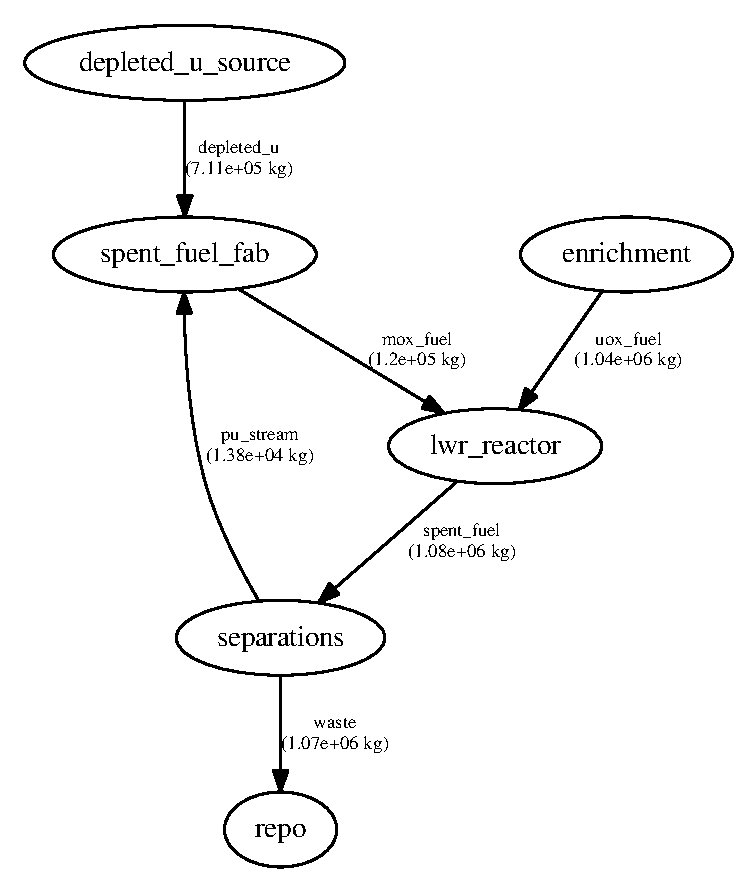
\includegraphics{./images/flow-closed-1.eps}
\end{center}
\caption{Full \gls{MOX} recycle (multi-pass) fuel cycle material flows.}
\label{fig:flowclosed}
\end{figure}

Figure \ref{fig:puseries1} shows the full-system plutonium buildup for once
through (no recycle), 1-pass recycle, and infinite-pass recycle variations of
the one-reactor scenario described above. The figure was generated directly
from \Cyclus output data. After several batch cycles (near month 300) in the
1-pass and infinite-pass cases, enough separated fissile material accumulates
in the fuel fabrication facility to generate a full recycled batch.  When this
batch is transmuted, more plutonium is burned than created.  This results in a
drop in the total fuel cycle system plutonium inventory.  This pattern repeats
roughly every 10 cycles (200 months) for the 1-pass recycle case and every 9
cycles (180 months) for the infinite-pass recycle case.  Because the 1-pass
recycle scenario does not re-recycle material, it takes the fabrication
facility 2 cycles longer to accumulate a full batch of fissile material.

Because facilities are represented individually and transact discrete
materials as discrete events, realistic non-uniform patterns in facility
behavior that affect total system behavior are observed using \Cyclus.

\begin{figure}[H]
\begin{center}
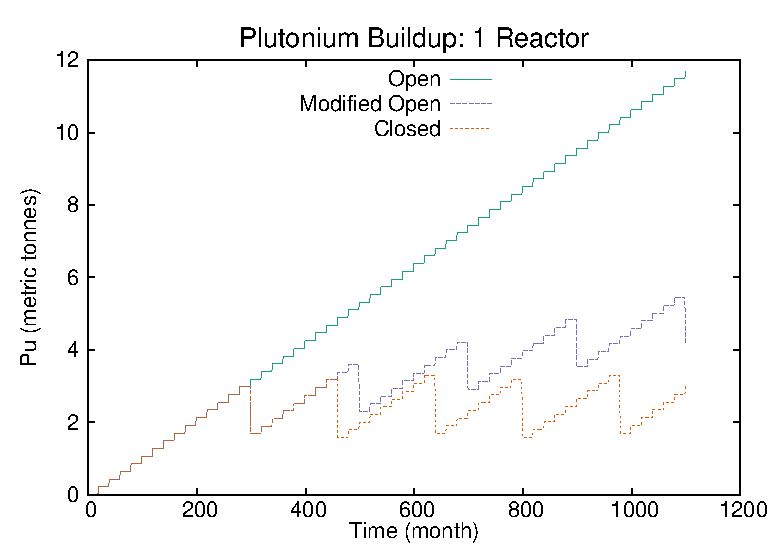
\includegraphics{./images/puseries-1.eps}
\end{center}
\caption{System plutonium buildup with one reactor.}
\label{fig:puseries1}
\end{figure}

Figure \ref{fig:puseriesn} shows plutonium buildup for the 10-reactor
simulations of the once through, 1-pass recycle, and infinite-pass recycle
scenarios.  As the number of reactors (with staggered refueling) increases,
the behavior of the system approaches a more steady average reminiscent of
continuous material flow models.

\begin{figure}[H]
\begin{center}
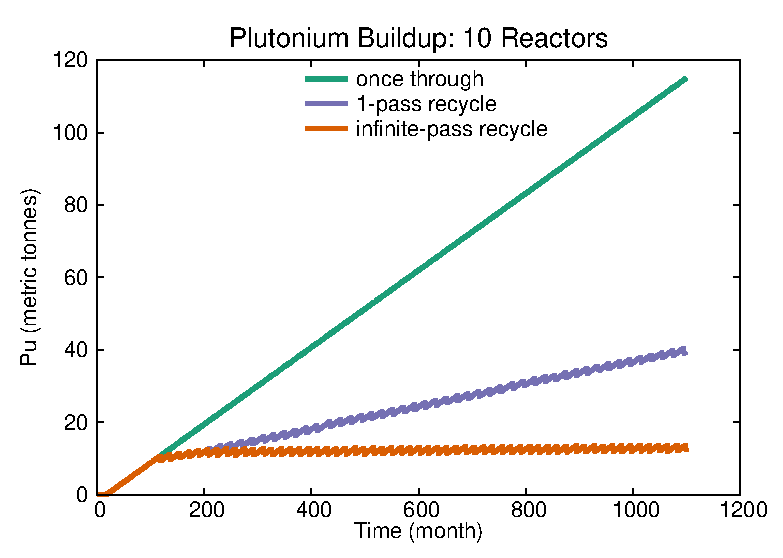
\includegraphics{./images/puseries-n.eps}
\end{center}
\caption{System plutonium buildup with staggered refueling for many reactors.}
\label{fig:puseriesn}
\end{figure}

The fundamental capabilities of demonstrated in these simulations qualify
\Cyclus and its ecosystem to model the breadth of scenario types expected of
nuclear fuel cycle simulator tools. These examples further show the flexibility
provided by the \gls{DRE} logic within the \Cyclus framework and provide
an example of the resolution made possible by discrete-facility and
discrete-material modeling in fuel cycle simulation.
